
\documentclass[a4paper,11pt,final,oneside,openright]{book}
\usepackage{rapport}

\newcommand{\reporttitle}{Développement Orienté Objet}
\newcommand{\enseignants}{Christine~\textsc{Solnon}\\ Elöd~\textsc{Egyed-Zsigmond}}
\newcommand{\reportauthor}{Guillaume~\textsc{Abadie}\\ Nicolas~\textsc{Buisson}\\ Louise~\textsc{Crépet}\\ Rémi~\textsc{Domingues}\\ Aline~\textsc{Martin}\\ Martin~\textsc{Wetterwald}}
\newcommand{\hexanome}{H4404}
\newcommand{\reportsubject}{Livrable de projet}
\newcommand{\dateperiod}{du 27 novembre au 20 décembre 2013}
\newcommand{\HRule}{\rule{\linewidth}{0.5mm}}
\setlength{\parskip}{1ex} % Espace entre les paragraphes

\hypersetup{
    pdftitle={\reporttitle},%
    pdfauthor={\reportauthor},%
    pdfsubject={\reportsubject},%
    pdfkeywords={INSA Lyon} {mot1} {mot2} {mot3}
}

\title{\reporttitle}
\author{\reportauthor}

%\setcounter{tocdepth}{4}
\begin{document}
    \renewcommand{\chaptername}{} %\renewcommand{\thechapter}{}
    \renewcommand{\contentsname}{Sommaire}

	\glsaddall
	\renewcommand{\chaptername}{}
	\renewcommand{\glossaryname}{Glossaire}

    \pagestyle{empty}
    \pagenumbering{Roman}
    % Inspiré de http://en.wikibooks.org/wiki/LaTeX/Title_Creation
\begin{center}
	\begin{minipage}[t]{0.48\textwidth}
	  \begin{flushleft}
	    
\includegraphics [width=40mm]{images/logo_INSA.png} \\[0.5cm]
			INSA Lyon\\
			20, avenue Albert Einstein\\
			69621 Villeurbanne Cedex
	  \end{flushleft}
	\end{minipage}
	\begin{minipage}[t]{0.48\textwidth}
	  \begin{flushright}
	    %\includegraphics [width=60mm]{images/logo_Passau.jpg} \\[0.5cm]
	    %Universität Passau\\
		%Innstraße, 3\\
		%	D-94032 Passau
	  \end{flushright}
	\end{minipage} \\[2cm]

	\textsc{\Large \reportsubject}\\[0.3cm]
	\HRule \\[0.4cm]
	{\Huge \bfseries \reporttitle}\\[0.6cm]
	{\Large \dateperiod}\\[0.4cm]
	\HRule \\[1cm]

	
\includegraphics [scale=0.55]{images/livraison.jpg} \\[0.7cm]
	\begin{minipage}[t]{0.4\textwidth}
	  \begin{flushleft} \large
	    \emph{Hexanôme \textbf{\hexanome}~:}\\
	    \small \reportauthor
	  \end{flushleft}
	\end{minipage}
	\begin{minipage}[t]{0.5\textwidth}
	  \begin{flushright} \large
	    \emph{Enseignants~:} \\
	    \enseignants
	  \end{flushright}
	\end{minipage}

	\vfill
	\footnotesize{Année scolaire 2013-2014}
\end{center}

    \sloppy          % Justification moins stricte : des mots ne dépasseront pas des paragraphes

    \frontmatter
    \pagestyle{empty}
    \tableofcontents
    \addtocontents{toc}{\protect\thispagestyle{empty}}

    \mainmatter
    \pagestyle{headings}
	\renewcommand{\chaptermark}[1]{\markboth{\MakeUppercase{#1}}{}}
	\renewcommand{\sectionmark}[1]{\markright{#1}}
	\chapter*{Introduction}
\addcontentsline{toc}{chapter}{Introduction}
\chaptermark{Introduction}

Ce dossier a pour but de vous présenter le sytème de gestion des livraisons du Grand Lyon, Optifret\textunderscore COURLY.
Nous nous attarderons ici plus spécifiquement sur l'interface du superviseur, qui lui permet de gérer les demandes de
livraisons des clients utilisant le système.

Vous retrouverez dans ce dossier la démarche détaillée de la capture et de l'analyse des besoins, ainsi que la
description complète de la conception de l'application. Nous espérons que notre système Optifret\textunderscore COURLY vous donnera
une entière satisfaction.



    \renewcommand{\chaptermark}[1]{\markboth{\MakeUppercase{\chaptername\ \thechapter.\ #1}}{}}
    \renewcommand{\sectionmark}[1]{\markright{\thesection{} #1}}

    \chapter{Mod\`ele du domaine}

\begin{figure}[h]
    \centering
    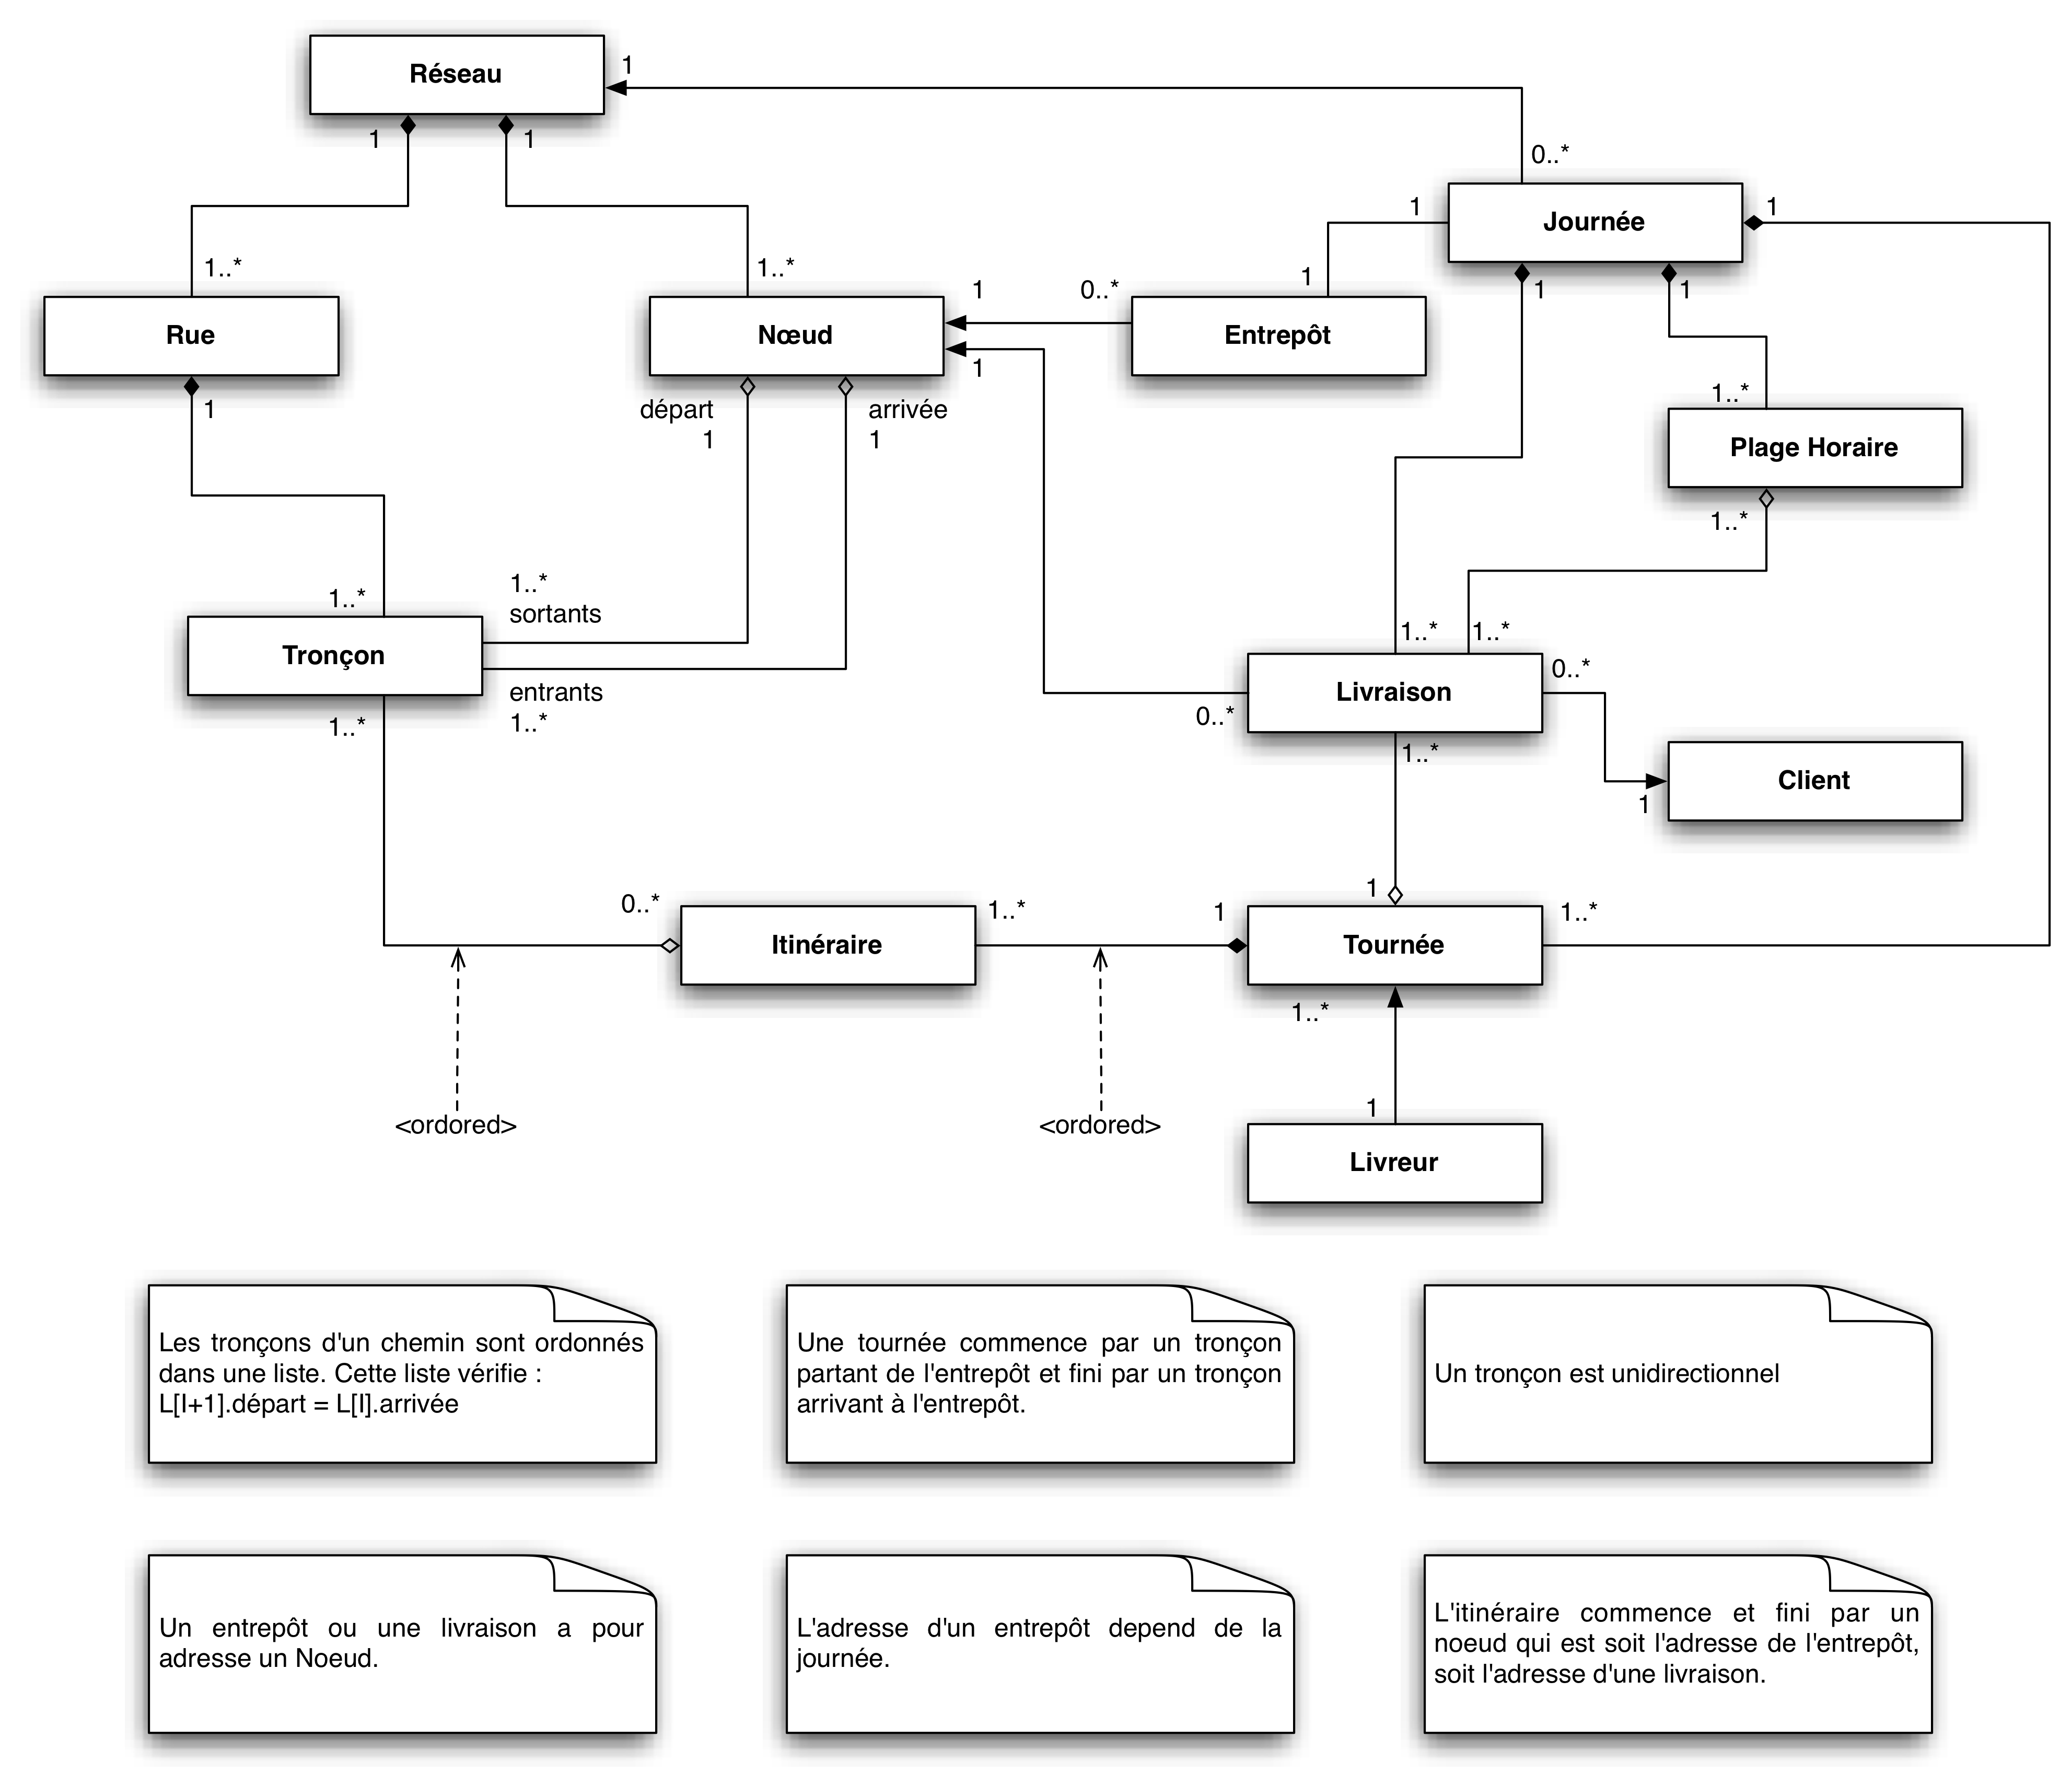
\includegraphics[width=140mm]{../diagrams/domain_model/domaine.png}
    \caption{Mod\`ele du domaine}
    \label{diagram:domaine}
\end{figure}


	\renewcommand{\chaptermark}[1]{\markboth{\MakeUppercase{#1}}{}}
	\renewcommand{\sectionmark}[1]{\markright{#1}}
	\chapter*{Conclusion}
\addcontentsline{toc}{chapter}{Conclusion}
\chaptermark{Conclusion}
Ceci est ma conclusion.


    \backmatter
	\phantomsection
	\addcontentsline{toc}{chapter}{\glossaryname}
	\printglossary[title=\glossaryname]
\end{document}
